\documentclass{article}

\usepackage[UTF8]{ctex}
\usepackage{amsmath}
\usepackage{graphicx}


\title{目标检测相关细节}
\author{叶亮}
\date{\today}
\begin{document} 
\maketitle
\section{Loss}
\subsection{IoU loss}


\subsection{GIoU loss}

\subsection{DIoU loss}

Code optimization, the calculation of distance between two center points of bboxes.
\begin{equation}
\begin{aligned}
(C_1-C_2)^2)&= ((x1_{C1}+x2_{C1})/2-(x1_{C2}+x2_{C2})/2)^2 \\
&=((x1_{C1}+x2_{C1})-(x1_{C2}+x2_{C2}))^2/4 \\
\end{aligned}
\end{equation}
\subsection{CIoU loss}
\subsection{BIoU loss}

\section{bbox \& anchor}

\subsection{coder}
在RetinaNet、SSD、Cascade R-CNN等网络中,网络预测的bbox都会进行Delta xywh编码,即将原始的(xmin, ymin, xmax, ymax)进行编码,计算相对距离,来减小回归的过拟合,提升回归的稳定性。
\begin{equation}\textbf{•}
\begin{aligned}
&\delta_x = (g_x-p_x)/p_w	   & \delta_y = (g_y - p_y)/p_h \\
&\delta_w = \log{g_w/p_w}	&\delta_h = \log{g_h/p_h}
\end{aligned}\label{bbox_coder}
\end{equation}

上述公式计算得到的$\delta$值通常很小,因为网络通常只对p进行少量微调,导致回归loss比分类loss小很多。为了提升学习的有效性,$\delta$通常需要经过均值和方差进行标准化.

\begin{equation}
\begin{aligned}
\delta_{x}^{'}=\frac{\delta_x-\mu_x}{\rho_x}
\end{aligned}
\end{equation}

\section{training}
\subsection{Optimizer}
\subsubsection{warmup}
warmup通常有三个方式:linear, constant, exp. 通常需要设置warmup的迭代数$iter_{total}$和warmup的增加比率ratio,
\begin{align}
lr_t = lr_{constant}*ratio
\end{align}
\begin{equation}
\begin{aligned}
lr_t = lr_{const}*(1-k), \\
k= (1-iter_t /iter_{total}) * (1-ratio)
\end{aligned}
\end{equation}
\begin{align}
lr_t = lr_{const}*k, \\
k=ratio^{1-iter_t/iter_{total}}
\end{align}

\section{Yolov4}
Yolov4的实现过程中,anchor的生成以及label与anchor的对应关系的构建方法。
\subsection{Anchor generation \& target build}
与retinanet,rcnn系列等bbox预测不同的是,yolo模型推理得到的结果(x,y,w,h)需要经过如下公式进行编码:
\begin{equation}
\begin{aligned}
b_x=\rho(t_x)+c_x
\end{aligned}
\end{equation}
\begin{figure}
\centering
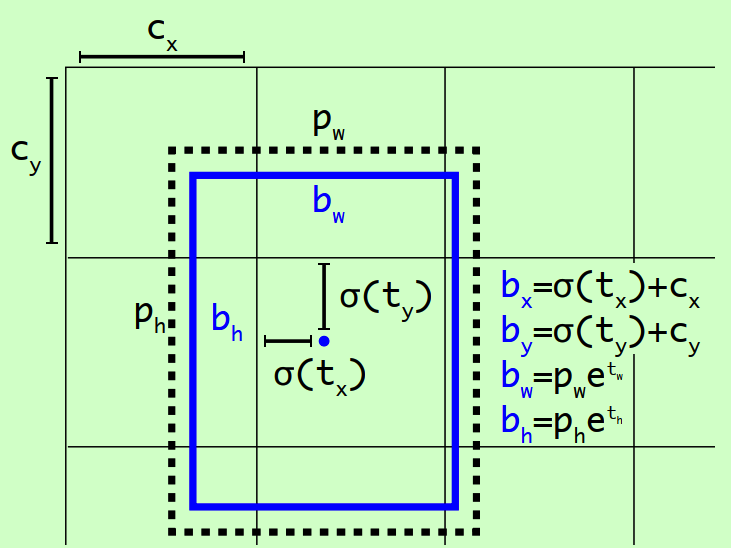
\includegraphics[scale=0.5]{images/yolo_bbox.png}
\caption{Yolo bbox prediction}
\end{figure}

\section{backbone}
\subsection{Regularization}
\subsubsection{Dropout}
原理,dropout随机丢弃神经元(全连接中输入神经元),实现方式为$keep_prob$,每个神经元生成一个随机数$k,k<keep_prob$即丢弃。优点,该方法有利于分类中泛化能力的提升.
\subsubsection{Drop Connect}
\subsubsection{Drop block}

\section{Refinedet}
\subsection{Anchor}
Refine中的anchor计算。对于每一个feature map, 首先计算其mesh grid,然后计算每个框的中心点$(x,y)=((i+0.5)/featsize,(j+0.5)/featsize)$,然后根据每个feature map对应的anchor box的大小,计算anchor的长和宽$WH_{ki}=box_k/imagesize, where k means kth feature level, i means ith grid$. e.g, 使用四个feature level, $box=[32,64,128,256], imagesize=320, featsize=[40,20,10,5], aspect ratio=[2,2,2,2]$, 那么最终生成$40*40*3+20*20*3+10*10*3+5*5*3=6375$个anchor.
\end{document}

